\section{Compiler heap}

We must think about when frontend releases the memory
or whether doesn't release it forever,
which is allocated by dynamic memory allocation routine
{\tt{malloc}} or {\tt{new}} etc.
Because it depends on speed and correctness of compiler.

For some object which is placed after frontend allocates memory,
we'll discuss the object is permanent or temporary.
Everything outside any function is permanent.
So discuss about inside function in later clause.

\subsection{Type}

In chapter \ref{type_e001}, we mentioned about the way of
representing type by {\em dag}.
If the type is already created and it exsits in type table,
frontend reuse it without creating again.
Please note that the type table may have temporary type
and frotned should relase the memory for it.
For example,
\begin{verbatim}
void f(void)
{
  struct S {
    ...
  };
  const struct S cs;
  struct S* ps;
  ...
}
\end{verbatim}
Frontend makes the scope corresponding function body `{\tt{f}}'
which contains a tag related with {\tt{struct\,\,S}}
and release the scope with them. i.e. {\tt{struct\,\,S}} is
temporary.

Frontend'll add type expression of {\tt{const\,\,struct\,\,S}}
into {\tt{const\_type}} type table, which was mentioned at
\ref{type_e002}. Frontend must release type expression and
erase it from the type table.

Similary, 
frontend will add type expression of {\tt{struct\,\,S*}}
into {\tt{pointer\_type}} type table, which was mentioned at
\ref{type_e003}. Frontend must release type expression and
erase it from the type table.

\subsubsection{Tagged types}

We discussed about these types at \ref{type_e010},
where they are related with a scope.
In {\tt{C}} language, it is possible to declare a tag
in function parameter scope.
\begin{verbatim}
struct S { long int x; unsigned char y[8]; };

void f(struct S { int a; double b; }* ps)
// Declaration `struct S' which is different with `::S'
{
  // ps->a, ps->b can be used.
}
\end{verbatim}
Even though function `{\tt{f}}' parameter scope is temporary,
it is incorrect to release the memory for {\tt{struct\,\,S}},
or to release the memory for pointer to {\tt{struct\,\,S}},
because function `{\tt{f}}' may be referenced until
the end of translation unit(file).

\subsection{Constant}

Depending on the implementation of frontend,
normal constants may be inserted in the global scope symbol table.
In such an implementation, temporary constants must not be
inserted in the global scope symbol table. For example,
\begin{verbatim}
void f(int n)
{
  struct S {
   ...
  };
  switch ( n ) {
  case (struct S*)0x2000 - (struct S*)0x1000:
  ...
  }
}
\end{verbatim}
in this case, frontend will generate constant pointers
which represent {\tt{(struct\,\,S*)0x2000}} or
{\tt{(struct\,\,S*)0x1000}}. And they must be
inserted in the function `{\tt{f}}' body symbol table.
And more, they must be relased after compilation function `{\tt{f}}'
is finished.

\subsection{Medium variables}

In figure \ref{expr_e013}, `{\tt{var}}' and other classes derived
from it are used for the result of evaluating an expression.
Almost all are inserted into symbol table, but 
`{\tt{addrof}}' are not inserted, or some implementation
doesn't insert something special into symbol table.
It is necessary to release the memory for
`{\tt{var}}' and other classes derived from it which doesn't exist
in symbol table.

\subsection{3 address code}
\label{speed3ac_e}
For easy, We didn't mention that
it is necessary to relase the memory for discarded
3 address codes. For example, when frontend
evaluates the result of {\tt{sizeof}} expression
which is applied to some expression,
\begin{verbatim}
var* sizeof_expr::eval()
{
  int n = code.size();
  var* expr = m_expr->eval();
  expr = expr->rvalue();

  // Release the memory for generated code before discarding them.
  for (auto p : code)
    delete p;

  code.resize(n);
  ...
  return expr->m_type->size();
}
\end{verbatim}
\subsection{Label}

At \ref{stmt_e000}, we mentioned about defined and used label tables.
And the tables must be cleared after an function compilation is finised.

\section{Backend symbol table traverse}
\label{speedback_e}
This contents are eliminated because it's old.

%% When frontend outputs symbol table and 3 address codes to backend,
%% backend must know the contents of symbol table before converts
%% 3 address codes to target processor assembly language.
%% 
%% Generally, symbol table is tree structure described at
%% \ref{symtab_e000}, but actually it is restricted tree
%% like figure \ref{speed_e000}.
%% 
%% \begin{figure}[htbp]
%% \begin{center}
%% \begin{htmlonly}
%% 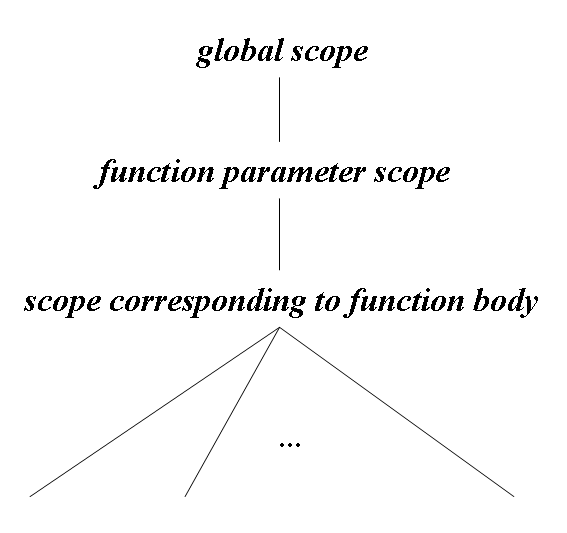
\includegraphics[width=0.5\linewidth,height=0.5\linewidth]{traverse_e.png}
%% \end{htmlonly}
%% \begin{latexonly}
%% 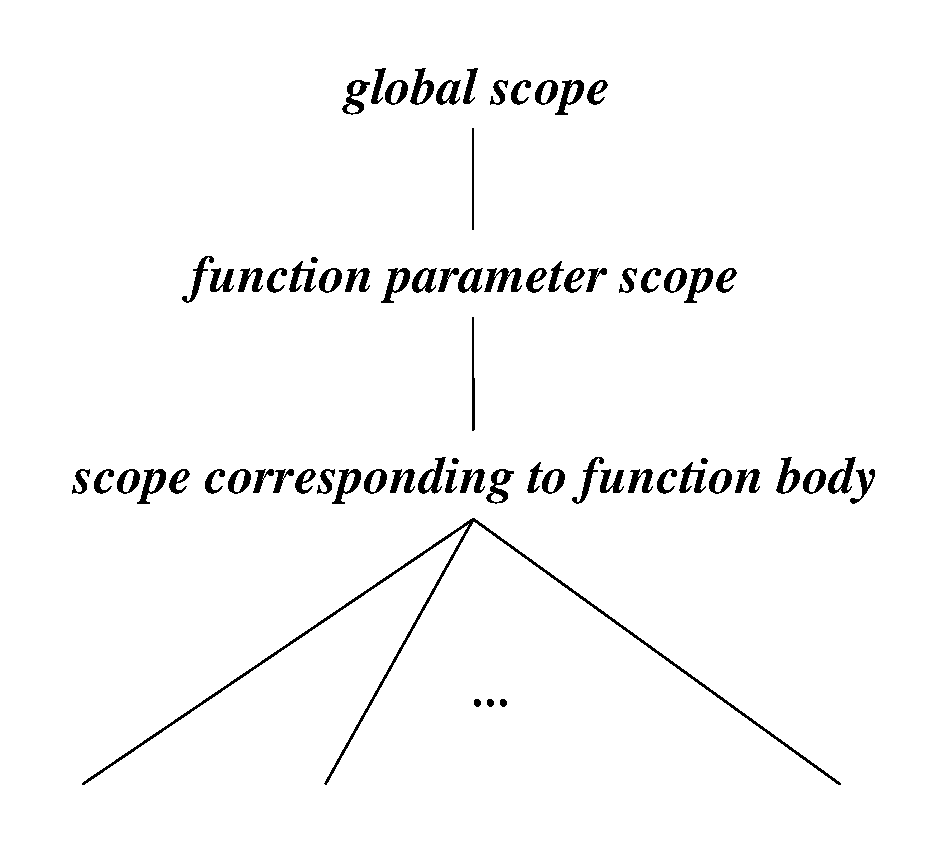
\includegraphics[width=0.5\linewidth,height=0.5\linewidth]{traverse_e.eps}
%% \end{latexonly}
%% \caption{Symbol table outputed by frontend to backend}
%% \label{speed_e000}
%% \end{center}
%% \end{figure}
%% 
%% Every scope except for ``global scope'' in figure \ref{speed_e000}
%% is outputed to backend differently with any time.
%% On the other hand, ``global scope'' becomes grater than
%% previous time. If a big translation unit (file) is
%% compiled, ``global scope'' increases.
%% 
%% Now, we want to deal with ``global scope'' specially.
%% Frontend prepares a container where only new entries exists,
%% backend referenses it like below.
%% \begin{verbatim}
%% // Frontend : Container for only new entries added into global scope.
%% vector<usr*> new_external_declaration;
%% 
%% // Frontend : routine for adding into symbol table
%% void add_symtab(usr* entry)
%% {
%%   string name = entry->m_name;
%%   map<string, vector<var*> >& usrs = scope::current->m_usr;
%%   usrs[name].push_back(entyr);
%%   if ( scope::current == &scope::root ) {
%%     // added into global scope
%%     new_external_declaration.push_back(entry);
%%   }
%% }
%% 
%% // Frontend : Yacc action function when grammer symbol
%% // `function-definition' is reduced.
%% void function_definition(comp_stmt* cs)
%% {
%%   cs->gen();  // 3 address codes are outputed in global
%%               // container `code'
%%   ...
%%   
%%   // Output symbol table, 3 address codes and new entries added
%%   // in global scope to backend
%%   backend(&scope::root,code,new_external_declaration,...);
%%   ...
%%   new_external_declaration.clear(); // Clear here.
%% }
%% 
%% // Backend : traverse symbol table
%% void traverse(scope* ptr)
%% {
%%   if ( ptr == &scope::root ) {
%%     // Global scope. Specially reference the container
%%     const vector<usr*>& v = new_external_declaration;
%%     for_each(v.begin(),v.end(),...);
%%   }
%%   else {
%%     // Not global scope. Normally reference symbol table.
%%     map<string, usr*>& usrs = ptr->m_usrs;
%%     for_each(usrs.begin(),usrs.end(),...);
%%     ...
%%   }
%%   vector<scope*>& children = ptr->m_children;
%%   for_each(children.beign(),children.end(),traverse);
%% }
%% \end{verbatim}
%% Internally, backend may have the table which converts `{\tt{var}}' to
%% address descriptor. In such an implementaion, the table should be
%% parted into permanent table and temporary table like below.
%% \begin{verbatim}
%% // Table converting var to address descriptor
%% typedef map<var*, address*> addr_desc;
%% 
%% pair<addr_desc,addr_desc> address_descriptors;
%% // Use address_descriptors.first as permanent and
%% // address_descriptors.second as temporary
%% \end{verbatim}

\section{{\tt{dynamic\_cast}}}

We use {\tt{C++}} language for implementing {\tt{C}} compiler.
And we use {\tt{dynamic\_cast}} in some situations.
Please remember that
this operator is very expensive judging from compile speed.

